%Present/motivate key ideas/decisions, design options, alternatives, trade-offs.
%Draw architecture block diagram (= picture!).

\subsection{Coefficient generator}
In order to avoid computing the filter coefficients on the board, we pre-compute them using a Java program (given in Appendix~\ref{app:source:generator}) and load them into the board's ROM.

We generate values for \texttt{lanczos2} from $-2.0$ to $2.0$, encode these float values as integers by multiplying them by $2^15$.
Then, we write them to a file as ASCII-encoded hexadecimal values.

\begin{figure}
	\centering
	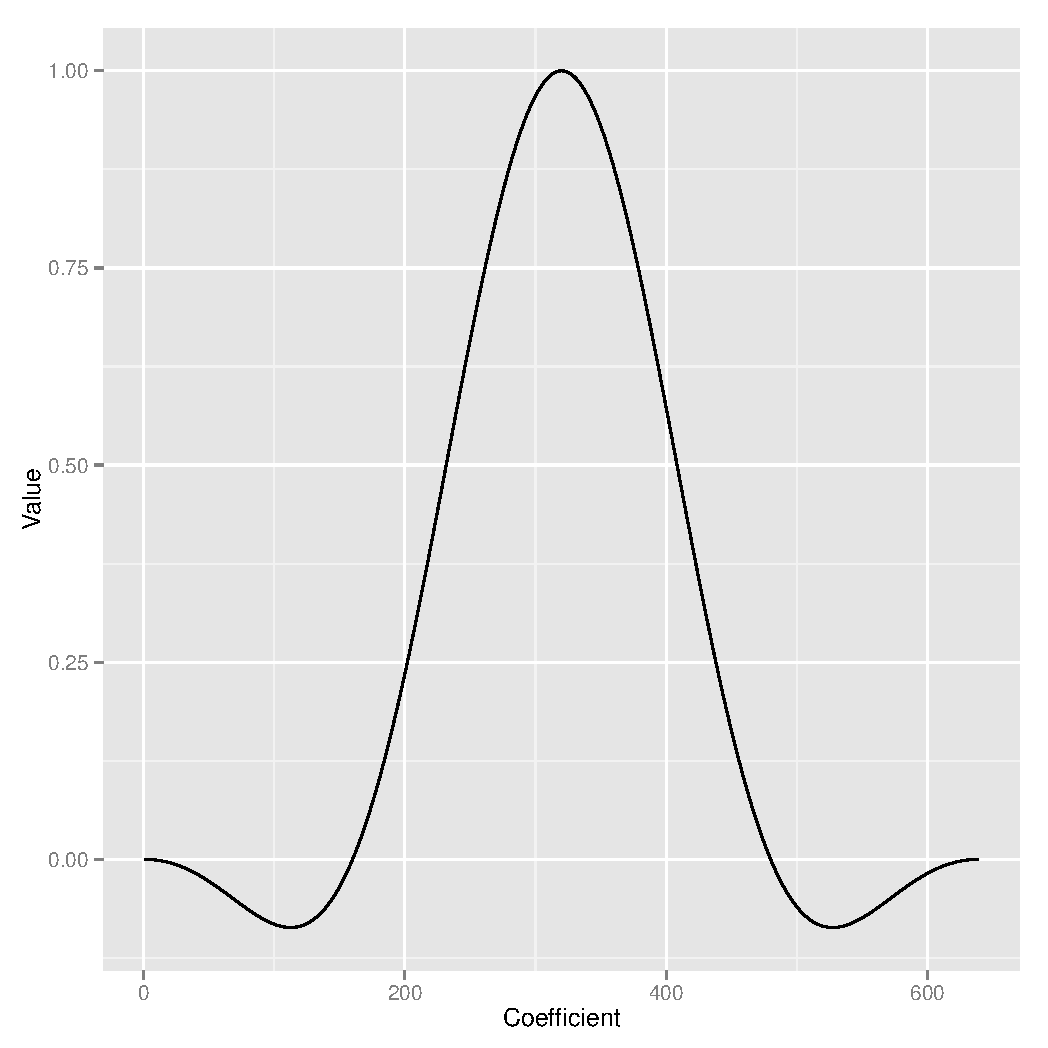
\includegraphics[width=0.5\textwidth]{coefficients}
	\caption{The coefficients generated by our program}
	\label{fig:coefficients}
\end{figure}

To make sure that our program returned the correct values, we made a plot of the output.
Figure~\ref{fig:coefficients} shows that plot, which is the result we expected.

\subsection{Filter}

Figure~\ref{fig:design:block} gives the block diagram for our design.

\begin{figure}[h]
	\centering
	\def\svgwidth{0.6\textwidth}
	\input{imgs/block.pdf_tex}
	\caption{Block diagram for our filter}
	\label{fig:design:block}
\end{figure}
